\documentclass[11pt]{article}
\usepackage{amssymb}
\usepackage{amsmath}
\usepackage{mathrsfs}
\usepackage{bbm}
\usepackage{tikz}
\usepackage{accents}
\usepackage[utf8]{inputenc}
\usepackage[english]{babel}
\usepackage{graphicx}
\usepackage{centernot}
\newcommand{\bs}{{\bigskip}}
\newcommand{\floor}[1]{\lfloor #1 \rfloor}
\newcommand{\ceiling}[1]{\lceil #1 \rceil}
\newcommand{\ms}{{\medskip}}
\newcommand{\sms}{{\smallskip}}
\newcommand{\N}{\mathbb{N}}
\renewcommand{\baselinestretch}{1.5}
\newcommand{\indi}{\mathbbm{1}}
\newcommand{\R}{\mathbb{R}}
\newcommand{\sigF}{\mathcal{F}}
\newcommand{\Z}{\mathbb{Z}}
\newcommand{\C}{\mathbb{C}}
\newcommand{\Q}{\mathbb{Q}}
\newcommand{\E}{\mathbb{E}}
\newcommand{\B}{\mathbb{B}}
\newcommand{\dd}[2]{\frac{d{#1}}{d{#2}}}
\newcommand{\fancyF}{\mathscr{F}}
\newcommand{\borelB}{\mathcal{B}}
\newcommand{\Var}{\text{Var}}
\newcommand{\inner}[2]{\langle{#1},{#2}\rangle}
\newcommand{\sinner}[1]{\langle{#1},{#1} \rangle}
\renewcommand{\epsilon}{\varepsilon}
\renewcommand{\overrightarrow}{\vec}
\newcommand{\tb}{\textbf}
\newcommand{\bfrac}[2]{\displaystyle{\frac{#1}{#2}}}
\newcommand{\bcup}{\bigcup\limits}
\newcommand{\bcap}{\bigcap\limits}
\newcommand{\ceil}[1]{\left\lceil #1 \right\rceil}
\newcommand{\nimply}{\centernot\Rightarrow}
\newcommand{\ar}{\Rightarrow}
\newcommand{\norm}[2]{\| #1 \|_{#2}}
\newcommand{\bnorm}[1]{\norm{#1}{}}
\newcommand{\probp}{\mathbb{P}}
\newcommand{\enorm}[1]{\| #1 \|}
\newcommand{\goto}{\rightarrow}
\newcommand{\bint}[2]{\displaystyle{\int_{#1}^{#2}}}
\newcommand{\nogoto}{\centernot\rightarrow}
\renewcommand{\baselinestretch}{1.5}
\newcommand{\bsum}[2]{\displaystyle{\sum_{#1}^{#2}}}
\newcommand{\bprod}[2]{\displaystyle{\prod_{#1}^{#2}}}
\newcommand{\func}[3]{#1: #2\rightarrow#3}
\newcommand{\sfunc}[2]{#1: #2\rightarrow#2}
\newcommand{\cexp}[2]{\E[#1 \mid #2]}
\usepackage{venndiagram}
\newcommand{\Lim}[1]{\raisebox{0.5ex}{\scalebox{0.8}{$\displaystyle \lim_{#1}\;$}}}
\newcommand{\Limn}{\Lim{n \in \N}}
\newcommand{\Cross}{\mathbin{\tikz [x=1.4ex,y=1.4ex,line width=.2ex] \draw (0,0) -- (1,1) (0,1) -- (1,0);}}
\title{ BA-Sindy}
\author{}
\setlength{\parindent}{0pt}

\begin{document}

\centerline{\tb{Sample results for PA-Sindy algorithm}}

Train data was of dimension $128 \times 32000$,  generated from Lorentz system.
Test data was of dimension $128 \times 5000$,  generated from same Lorentz system.
 Test loss values and coefficient counts for each averaged over 10 runs is given in the plots below.   ( sindy\_x loss is multiplied by weight hyper-param  $10^{-4}$)
 
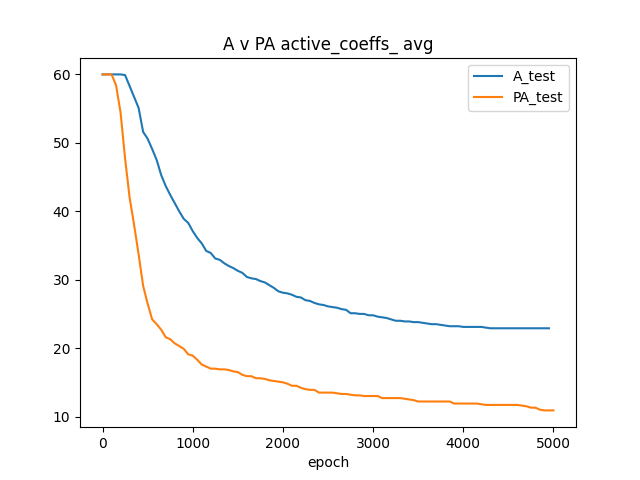
\includegraphics[width=85mm]{coeffs.png}
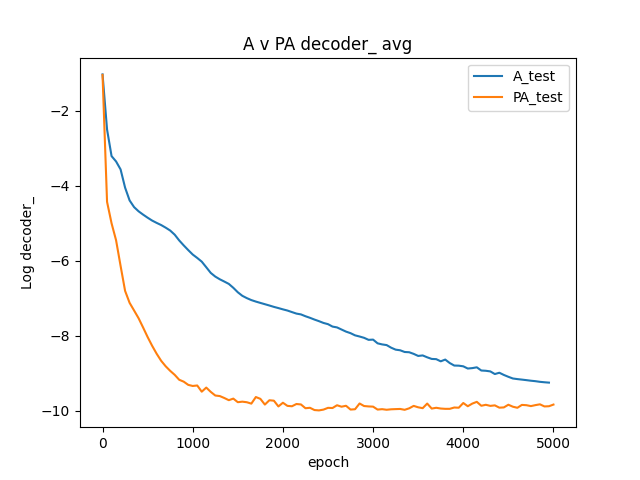
\includegraphics[width=85mm]{decoder.png}
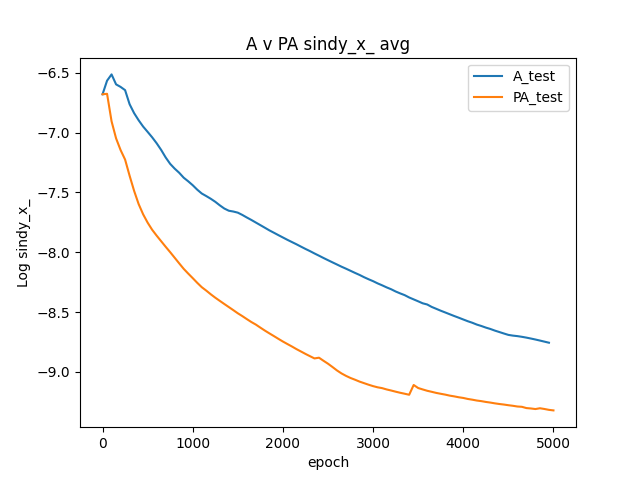
\includegraphics[width=85mm]{sindy_x.png}


\pagebreak

Next plots are same setup,  except the coefficient for the submodels are initialized randomly instead of uniformly to one.  Note we no longer achieve better sparsity but the sindy\_x loss is much much better than in the uniform initialization case.  The same does not hold for A-sindy with random initialization.  Random init of A-sindy yields better sparsity but worse Loss.


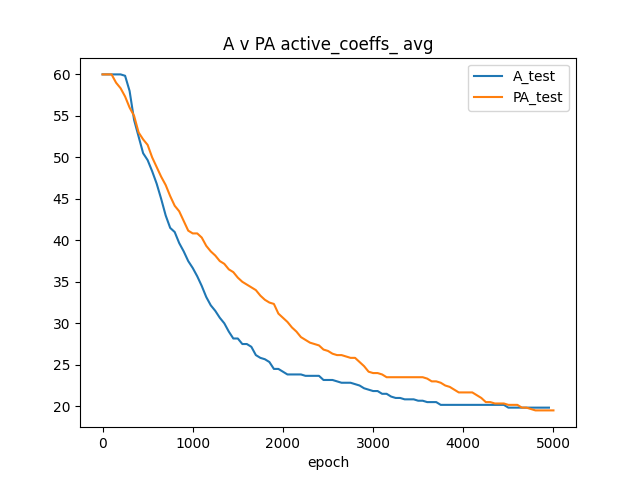
\includegraphics[width=85mm]{ri_coeffs.png}
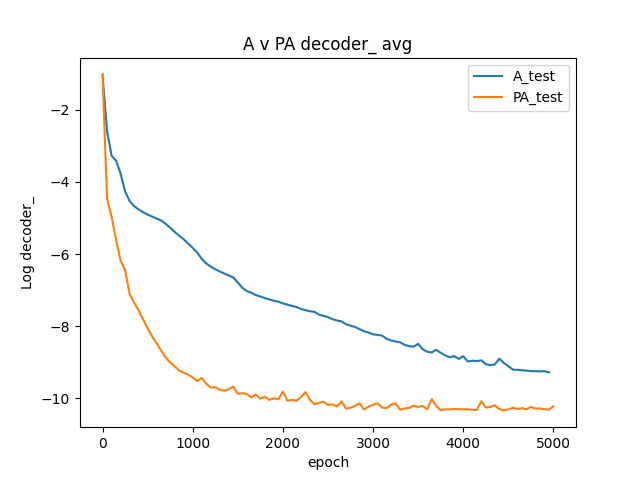
\includegraphics[width=85mm]{ri_decoder.png}
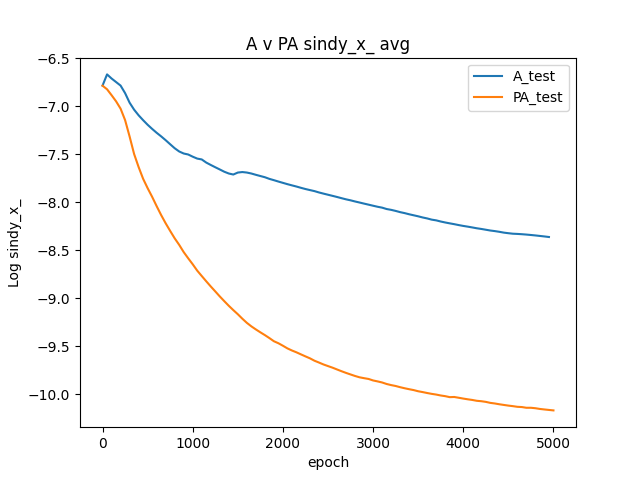
\includegraphics[width=85mm]{ri_sindy_x.png}

\end{document}

